%!TEX root =  GDELT_GA_Search_UsersManual.tex

\chapter{Introduction} \label{chap:Introduction}
\par GDELT is the Global Database of Events, Language, and Tone, a record of real-world events  harvested automatically from world news sources. Its records begin from 1979 and continue to the present, and the most recent versions of the GDELT data set are updated every 15 minutes. The records are compiled using natural language processing (NLP), and the record for each event includes not only information about the actors and actions, but also about aspects of how the action is described and discussed in the news: how widely, for how long, in what tone, etc. Consequently, GDELT provides an incomparable record of how events in the real world are being considered and expressed by the general public.

\par At a micro-level, a record in the GDELT data set is able to shed light on how a specific event was considered. For example, the GDELT data set shows whether an event was discussed widely or only briefly, whether it was discussed while it ocurred or only afterwards, whether it was debated or celebrated, or whether it was memorialized and recalled long after it first took place. At a macro-level, the complete record of GDELT events forms a richer data source, one that can inform about long-term dynamics and ongoing world historical processes, of which individual events are only single lines in a longer play.

\par A difficulty, however, is that the complete GDELT data set covers the whole world: it is more than just one play; it is a whole library. The challenge is often to find the correct level at which to understand the story that GDELT is telling. More formally, one might wish to isolate specific subsets of the GDELT data that apply to an area of interest and to leave out all of those that do not.

\par GDELT is integrated with a query search that can extract subsets based on the data contained in GDELT's records. For example, if one were interested in diplomacy between France and Russia in 2018, one could perform a search in which those two countries are listed as `actors' and the time range was limited to the period of interest of 2018. Other filters (for example, actions of specific kinds) could also be applied. However, for some purposes, it may be difficult to guess at what is the proper query because false positives and false negatives can dominate, washing out the signal.

\section{Finding Relevance: A GA Approach}

\par The \gdgas toolkit assumes that there can be valuable relationships between subsets of GDELT data and other time-series data found in the real world. The canonical example is that bursts of activity in global news reporting concerning some ongoing process (e.g., a world conflict) will be echoed by similar activity on social media platforms. Because of this relationship between news and social media, time-series showing activity on these social media platforms should be able to be related to a time-series showing discussions in world news events as catalogued by GDELT. 

\par An additional expectation is that these relationships will only be visible on specific subsets of the GDELT data. The global number of news articles collected by GDELT and the number of events catalogued will remain more or less constant, but the content will vary through time. The subset of content that is of interest will be unified by some common element such as a specific term, a set of terms, or even other criteria. The challenge is to find the criteria that, when issued as a query against the full GDELT data set, returns a set that has a signature related to the long-term issue being considered.

\par For example, the four graphs in figure \ref{FourGraphsFigure} show time series data with time on the x-axis. The upper graph represents the activity on some social media platform: activity is low early in the period shown, then there is a burst followed by heightened activity, and there is a drawdown through the remainder of the period.

\par The second graph from the top shows the total GDELT events. Note that this graph would already have been subselected using keywords. (Although the \gdgas toolkit can work with the entire GDELT data set, upstream preprocessing like this is common to winnow the GDELT data to only elements likely to be relevant.) The key aspect here is the alignment with the upper graph. Notice that there is a sharp burst and then a drawdown that shows a strong correlation between the graphs. Even so, the alignment is far from exact. (Note also that scales would be omitted from the axes. It is assumed that the x-axes are the same, but this is not true for the y-axis: the number of events in the upper graph may be in the millions while the number in the lower graph is in the thousands. What matters is their correlation.)

% re-do graph, needs to be a, b, c, and d of Fig. 1
% top graph maybe supposed to be SOCMED or SocMED? JTM: YES, it was supposed to be 'Social Media' or 'SocMed' or something...
% In this graph the match between top and bottom is perfect, because these are fake data, but if we re-do the graphs to use real data (hence imperfect) we can reword some of the description below. 
\begin{figure}
[htbp] 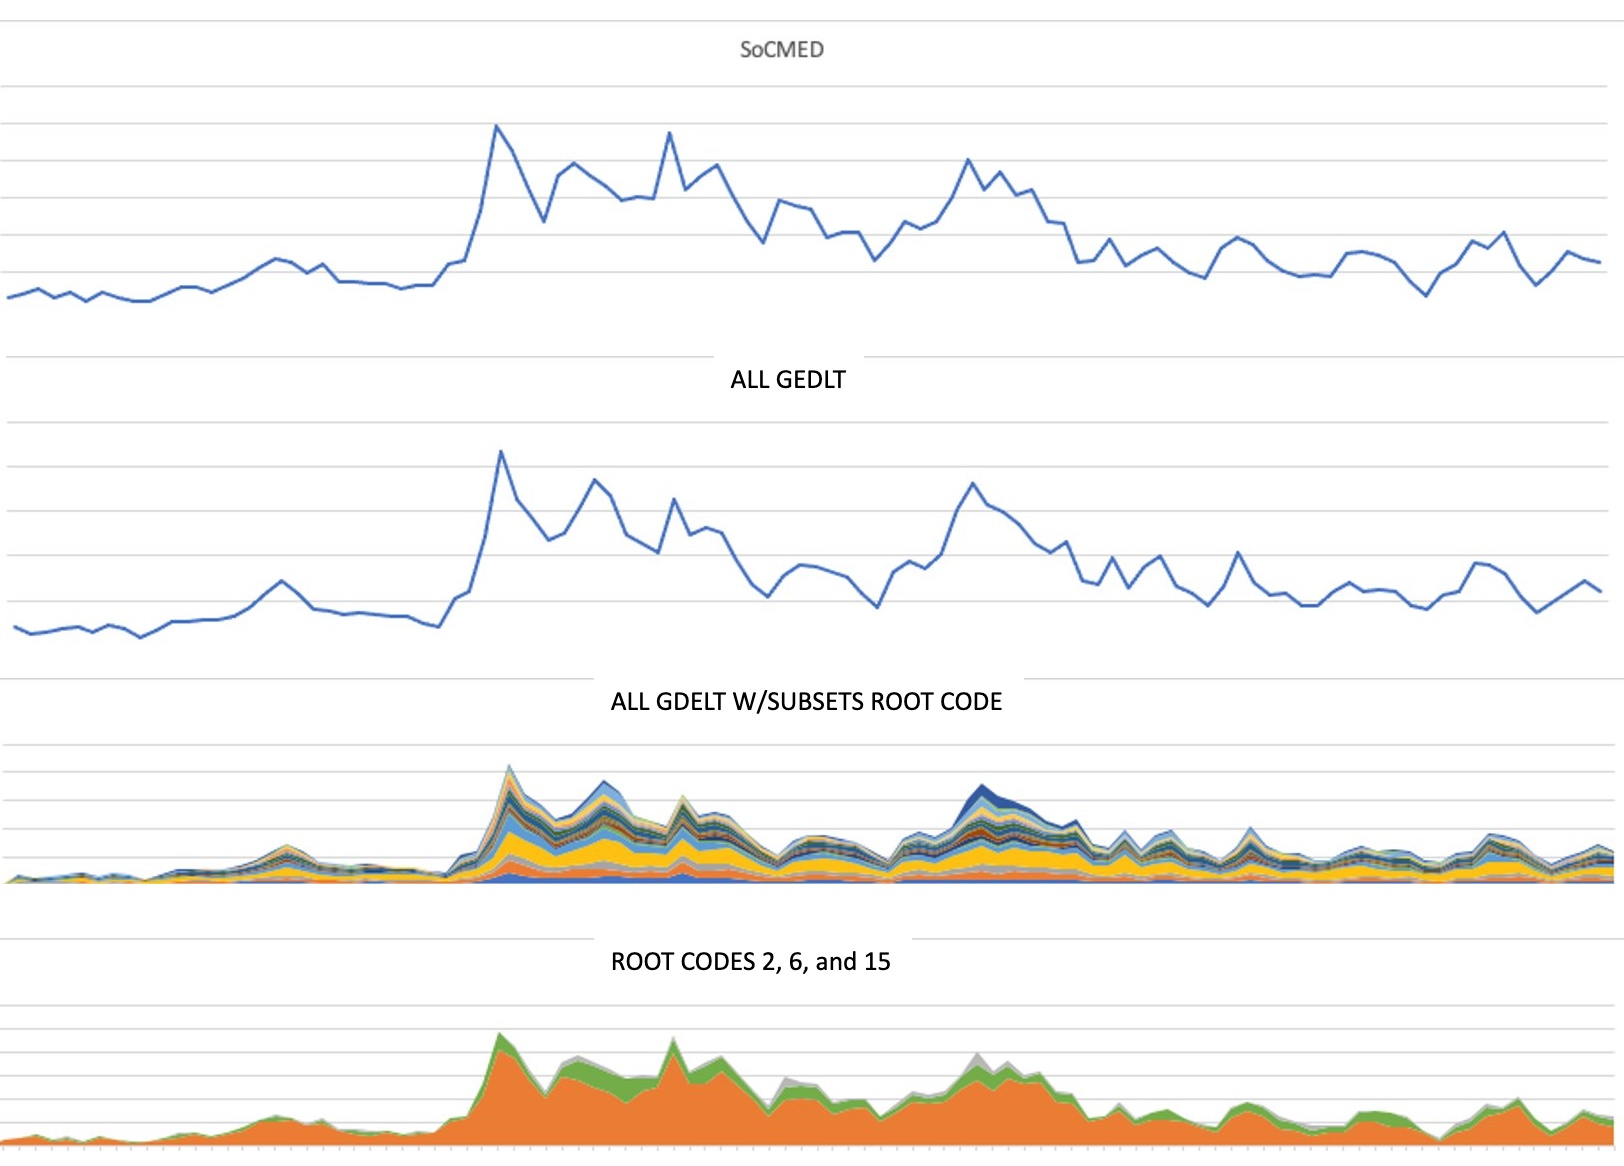
\includegraphics[width=\columnwidth]{TheoryGraphs.jpg}
\caption{Conceptual view of the search process} 
\label{FourGraphsFigure} 
\end{figure}

\par The ALL GDELT W/SUBSETS ROOT CODE graph (c) shows the same graph as (b); however, where (b) showed only the total, (c) subdivides the GDELT data---in this case, by the value for \textit{root code} (see below). There are 20 possible values for this field, and hence 20 bands in the graph. Each band represents the counts of GDELT events with the specified root code. 

\par The lowest graph (d) shows the results when only three root codes (2, 6, and 15) are included in the GDELT totals. Whereas the graph of all the GDELT events matches the social media event graph at a general level, the graph of these three specific root codes matches much more closely. 

\par This offers a nice example the \gdgas toolkit because it is easily bounded: with 20 root codes, there are exactly ${2^n - 1}$ combinations possible. For 20 root codes this is 1,048,575 combinations. This would be manageable with a brute-force approach---it is not difficult to try 1 million combinations---but this number grows quickly as more possible criteria are added. It is easy to reach a space that is too large to explore fully, so a different approach is needed instead.

\par The \gdgas tool searches through this space by building GDELT time series using \textit{queries}. A query is a set of criteria that serve to classify the GDELT data and extract matching events. The crux of the \gdgas algorithm is that these queries can be changed in an iterative way that moves through the search space. The algorithm is this:

\begin{itemize} 
	\item \textbf{Construct a query framework} that extracts subsets of GDELT data based on an array of possible fields 
	\item \textbf{Score the results} based on the information they provide about the social media time series
	\item \textbf{Mutate the best-scoring variations} to explore whether expanding or reducing the criteria improve the scores
\end{itemize}


\section{Acknowledgements}
%specific text that we have to use to acknowledge funders
%The funders (DARPA), the creators, the team, etc.


% Note: GDELT documentation indicates that some events are reciprocal: "Biden meets with Putin" would have a matching event, "Putin meets with Biden." These should show up as identical events but with the actors reversed; see https://www.gdeltproject.org/data/documentation/CAMEO.Manual.1.1b3.pdf, p. 8, CAMEO '019', "Express Accord". I have never found an example of this; GDELT does not link these together (they would be separate records), and it is unclear if every entry in the 'mentions' table would be duplicated as well.



% Let's save all of this for later in the document
% \par Test history is taken from 'test unknown'. See how good it does scoring things more than once to be sure it does not do well once by chance. %scoring what?
% \\The genetic algorithm operates through iterations. Iterations are given graph improvement scores over run-time. This is because there is a cost-benefit analysis for continuing to run. %make more clear
%Not sure what was planned below, plus hypperrefs don't work. 
%\par  \hyperref[sec:4]{To construct a query framework}
% \\Queries are methods of passing through data and finding subsets. Queries can contain other queries and the results can be added together and weighted.
%\par \hyperref[sec:3]{To construct a query framework} to score the results %add
%\par To mutate the best-scoring variations%add



% Let's also save this for later in the document
% Some fields \textit{completely determine others in the entire GDELT data set}. 
% For example, \emph{MonthYear} is merely a reformatted version of \emph{day}; whereas \emph{day} is in YYYY-MM-DD format, \emph{MonthYear} is in YYYYMM format. 
% So, if \emph{day} is known, then \emph{MonthYear} can be derived. 
%In many cases, searching on both fields would be redundant (although it may also be the case that a combination of search strategies might be better than searching just one field using one strategy).

% It may also be the case that some fields completely determine others \textit {within a specific subset of GDELT data}. For example, if a data set is drawn from a date range that begins %December 1st of 2010 and ends January 31st of 2011, then any record with a \emph{Year} value of 2010 must have a \emph{MonthYear} value of ``201012", and any record with a \emph{Year} value of 2011 must have a \emph{MonthYear} value of ``201101''. This, however, is an attribute of the subset of data use rather than the way that the GDELT data set has been constructed. It may be useful in specific applications, but not in the general case, it is not addressed further here.
